\section{Folgen und Reihen}

\subsection{Folgen}

\begin{definition}{Folgen}
    \begin{itemize}
  \item $n \in \mathbb{N}^{*} \rightarrow a_{n} \in \mathbb{R}$
  \item $\left(a_{k}\right)=\left(a_{k}\right)_{k \geq 1}=\left(a_{1}, a_{2}, a_{3}, \ldots, a_{n}, a_{n-1}, \ldots\right)$
\end{itemize}

Die Elemente einer Folge heissen Glieder der Folge $\rightarrow a_{n}$.
\end{definition}

\begin{definition}{Teilfolgen}
    Eine \emph{Teilfolge} einer Folge $\sequence$ ist eine Folge $\sequence[b]$ wobei $b_n = a_{l(n)}$ und $l: \N^* \to \N^*$ eine Abbildung mit der Eigenschaft: $l(n) < l(n+1)~\forall n \geq 1$.
\end{definition}

\begin{definition}{Monotonie}
    \begin{enumerate}
        \item $\sequence$ \emph{monoton wachsend} falls: \null\hfill $a_n \leq a_{n + 1} \quad \forall n \geq 1$.
    	\item $\sequence$ \emph{monoton fallend} falls: \null\hfill $a_n \geq a_{n+1} \quad \forall n \geq 1$.
    \end{enumerate}
\end{definition}

\begin{formula}{Wichtige Folgen}\\
    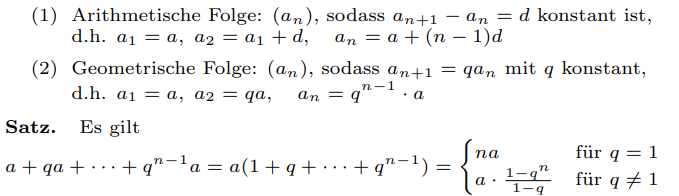
\includegraphics[scale=0.5]{wichtige_folgen.png}
\end{formula}

\begin{remark}
    Folgend sind diese Konzepte beispielhaft vereinfacht.\\
    Abkürzungen
    \begin{itemize}
      \item $A=$ Anfangs-Glied
      \item $d=$ Differenz
      \item $q=$ Quotient
    \end{itemize}
\end{remark}

\begin{definition}{Arithmetische Folge}
$$
a_{k}=(2,3,4,5, \ldots) \rightarrow d=1, A=2
$$

N-tes Glied

$$
a_{n}=A+(n-1) \cdot d
$$

Mittelwert

$$
a_{k}=\frac{a_{k-1}+a_{k+1}}{2}
$$

Partial-Summe

$$
S_{n}=n \cdot \frac{a_{1}+a_{n}}{2}=n \cdot\left(A+\frac{n-1}{2} \cdot d\right)
$$
\end{definition}

\begin{definition}{Geometrische Folge}
$$
a_{k}=\left(\frac{1}{1}, \frac{1}{2}, \frac{1}{4}, \frac{1}{8}, \ldots\right) \rightarrow q=\frac{1}{2}, A=1
$$

N-tes Glied
$$a_{n}=A \cdot q^{n-1}=\frac{A}{q} \cdot q^{n}$$

Mittelwert
$$
\left|a_{k}\right|=\sqrt{a_{k-1} \cdot a_{k+1}}
$$

Partial-Summe

$$
S_{n}=A \cdot \frac{1-q^{n}}{1-q}=A \cdot \frac{q^{n}-1}{q-1}
$$
\end{definition}

\subsection{Grenzwerte und Konvergenz von Folgen}

\begin{definition}{$\varepsilon$-Definition}
    \\Folge $\sequence$ heisst \emph{konvergent}, falls es $l \in \R$ gibt, sodass \vspace{1mm}

    $\forall \varepsilon > 0$ die Menge $\{n \in \N^* : a_n \notin~] l - \varepsilon, l + \varepsilon[\,\}$ endlich ist. ($\N^*$: $\N$/$0$.) \vspace{1mm} \\
    Einfach gesagt: das heisst, dass $|a_n - a| < \epsilon$ ab einem gewissen n für alle $\epsilon$ gilt.

\end{definition}

Bem: $l$ bezeichnet den Grenzwert $\lim_{n \to \infty} a_n$

\begin{definition}{Formelle Grenzwert Definition}
    Folgende Aussagen sind äquivalent:
    \begin{enumerate}
        \item $\sequence$ konvergiert gegen $l = \lim_{n \to \infty} a_n$
        \item $\forall \varepsilon > 0~\exists N \geq 1$, sodass $|a_n -l | < \varepsilon \quad \forall n \geq N$.
    \end{enumerate}
\end{definition}

\begin{lemma}{Einzigartigkeit Grenzwert}
     Es gibt max. ein $l \in \R$ für $a_n$ mit dieser Eigenschaft (max. 1 Grenzwert)
\end{lemma}

\begin{theorem}{Rechenregeln mit Folgen}
    \\Sei $\sequence,\sequence[b]$ konvergente Folgen mit$a = \lim_{n \to \infty} a_n$, $b = \lim_{n \to \infty} b_n$
    \begin{enumerate}
        \item $(a_n \pm b_n)_{n \geq 1}$ konvergent, $\lim_{n \to \infty} (a_n \pm b_n) = a \pm b$.
        \item $(a_n \cdot b_n)_{n \geq 1}$ konvergent, $\lim_{n \to \infty} (a_n \cdot b_n) = a \cdot b$.
        \item $(a_n \div  b_n)_{n \geq 1}$ konvergent, $\lim_{n \to \infty} (a_n \div b_n) = a \div b$.
        \\(solange $b_n \neq 0 ~ \forall n \geq 1$ und $b \neq 0$)
        \item Falls $\exists K \geq 1$ mit $a_n \leq b_n ~ \forall n \geq K$ folgt $a \leq b$.
    \end{enumerate}
\end{theorem}

\begin{highlight}{Spezielle Grenzwerte von Folgen}
    \tcbsubtitle{$n \to \infty$}
    \begin{equation*}
        n^x q^n \to 0 \quad \forall x \in \Z~\text{und}~0 \leq q \leq 1
    \end{equation*}
    \begin{equation*}
         n(\sqrt[n]{x} - 1) \to \ln x \quad \forall x>0
    \end{equation*}
    \begin{equation*}
        \sqrt[n]{a_n} \to 1 ~\text{wenn}~ \lim_{n \to \infty} a_n > 0 ~\text{und}~ \forall a_n > 0
    \end{equation*}
    \begin{center}
        \begin{minipage}{0.3\linewidth}
            \begin{align*}
                \frac{1}{n} &\to 0\\
                1 + \frac{1}{n} &\to 1\\
                \frac{2n}{2^n} &\to 0\\
                \sqrt[n]{n} = n^{\frac{1}{n}} &\to 1\\
                \sqrt[n]{n!} &\to \infty\\
                \frac{1}{n}\sqrt[n]{n!} &\to \frac{1}{e}\\
                \frac{x^n}{n!} &\to 0\\
                \frac{n^n}{n!} &\to \infty
            \end{align*}
        \end{minipage}
        \hfill\vline\hfill
        \begin{minipage}{0.3\linewidth}
            \begin{align*}
                e^n &\to \infty\\
                e^{-n} &\to 0\\
                \frac{e^n}{n^x} &\to \infty\\
                \frac{\sin n}{n} &\to 0\\
                \arctan n &\to \frac{\pi}{2}\\
                ln(n) &\to \infty\\
                \frac{ln(n)}{n} &\to 0\\
                \frac{log(n)}{n - 1} &\to 1
            \end{align*}
        \end{minipage}
        \hfill\vline\hfill
        \begin{minipage}{0.3\linewidth}
            \begin{align*}
                \forall k \in \Q^+ \hspace{2mm}\frac{1}{n^k} &\to 0\\
                \left(1 + n\right)^{\frac{1}{n}} &\to 1\\
                \left(1 + \frac{1}{n}\right)^x &\to 1\\
                \left(1 + \frac{1}{n}\right)^n &\to e\\
                \left(1 + \frac{x}{n}\right)^n &\to e^x\\
                \left(1 - \frac{1}{n}\right)^n &\to \frac{1}{e}\\
                \left(\frac{n}{n + x}\right)^n &\to e^{-x}
            \end{align*}
        \end{minipage}
    \end{center}
    \tcbsubtitle{Divergente Folgen}
    \begin{align*}
        &a_{n}=(-1)^{n}=(-1,1,-1,1,-1 \ldots) \\
        &a_{n}=3+2 n=(5,7,9,11, \ldots)
    \end{align*}
\end{highlight}

\subsection{Tricks und Strategien für Folgen}

\begin{KR}{Konvergenz Folgen}
    \begin{enumerate}
        \item Für Brüche, grösste Potenz von n ausklammern und kürzen. Alle übrigen Brüche der Form $\frac{a}{n^s}$ streichen, da diese zu 0 konvergieren.
        \item Für Wurzeln in einer Summe, multipliziere mit der Differenz der Summe (bei a + b multipliziere mit a - b)
        \item Anwendung Satz von Weierstrass
        \item Anwendung Sandwich-Satz
        \item Vergleich mit Referenz-Folgen (Spezielle Grenzwerte)
        \item Grenzwert durch simple Operationen und Umformen ermitteln
        \item Binom -, Substitutions-, Log-Trick?
        \item Definition der Konvergenz/Limes anwenden
        \item Suchen eines konvergenten Majoranten
    \end{enumerate}
\end{KR}

\begin{KR}{Divergenz Folgen}
    \begin{enumerate}
        \item  Suche einen divergenten Minoranten
        \item Für alternierende Folgen zeige, dass \\$\lim_{n \to \infty} a_p1(n) \neq \lim_{n \to \infty} a_p2(n)$
    \end{enumerate}
\end{KR}

\begin{KR}{Binom Trick}\\
    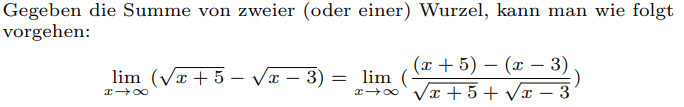
\includegraphics[scale=0.5]{binomtrick.png}
\end{KR}

\begin{KR}{Substitutions Trick}\\
    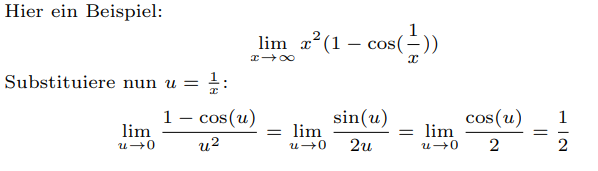
\includegraphics[scale=0.5]{substitutionstrick.png}
\end{KR}

\subsection{Satz von Weierstrass und Sandwich-Satz}

\begin{definition}{Supremum und Infimum}
    $A \subseteq \R, ~A\neq \emptyset$
    \begin{enumerateroman}
        \item $A$ nach oben beschränkt. Dann gibt es eine kleinste obere Schranke von $A$: $c \coloneqq \sup A$. Das \emph{Supremum} von $A$.
        \item $A$ nach unten beschränkt. Dann gibt es eine kleinste untere Schranke von $A$: $c \coloneqq \inf A$. Das \emph{Infimum} von $A$.
    \end{enumerateroman}
    \tcblower
    Vereinfacht formuliert: Für ein abgeschlossenes, halboffenes oder offenes Intervall $[a,b], [a,b), (a,b]$ oder $(a,b)$ gilt $inf = a$, $sup = b$ (solange $a, b \neq \infty$)
\end{definition}

\begin{concept}{Satz von Weierstrass}
    \begin{itemize}
        \item $\sequence$ monoton wachsend und nach oben beschränkt. $\Rightarrow$ $\sequence$ konvergiert mit $\lim_{n \to \infty} a_n = \sup \{a_n : n \geq 1\}$
        \item $\sequence$ monoton fallend und nach unten beschränkt. $\Rightarrow$ $\sequence$ konvergiert mit $\lim_{n \to \infty} a_n = \inf \{a_n : n \geq 1\}$
    \end{itemize}
\end{concept}

\begin{theorem}{Sandwich-Satz}
    Sei $\lim a_n = \alpha$ und $\lim c_n = \alpha$ und $a_n \leq b_n \leq c_n, \forall n \geq k$ dann gilt $\lim b_n = \alpha$\\
    Bmk: k steht hier für eine beliebige natürliche Zahl, ab der die Bedingung immer gilt. Also wie bei der Grenzwert-Definition mit dem <<Gürtel>> um den Grenzwert - das gilt ja auch erst ab einem gewissen Wert n.\\
    Bmk 2: Einfach gesagt heisst das, dass wenn wir den Grenzwert von zwei Folgen bereits kennen und dieser für beide gleich ist, und wir eine dritte Folge haben die <<zwischen>> die zwei bekannten Folgen passt (daher Sandwich-Satz), wissen wir dass auch die dritte Folge den gleichen Grenzwert wie die anderen zwei hat.
\end{theorem}

\subsection{Reihen}

\begin{definition}{Reihen-Konvergenz}
    Die Reihe $\sum_{k = 1}^\infty a_k$ ist \emph{konvergent}, falls die Folge $\sequence[S]$ der Partialsummen konvergiert. In diesem Fall definieren wir: $\sum_{k = 1}^\infty a_k \coloneqq \lim_{n \to \infty} S_n$
\end{definition}

\begin{theorem}{Rechenregeln von Reihen}
    \\Seien $\sum_{k=1}^\infty a_k$ und $\sum_{j=1}^\infty b_j$ konvergent, sowie $\alpha \in \C$.
    \begin{enumerate}
        \item Dann ist $\sum_{k=1}^\infty (a_k + b_k)$ konvergent.\\
            $\sum_{k=1}^\infty (a_k + b_k) = (\sum_{k=1}^\infty a_k) + (\sum_{j=1}^\infty b_j)$.
        \item Dann ist $\sum_{k=1}^\infty \alpha a_k$ konvergent. $\sum_{k=1}^\infty \alpha a_k = \alpha \sum_{k=1}^\infty a_k$
    \end{enumerate}
\end{theorem}

\subsection{Spezielle Reihen}

\begin{highlight}{Spezielle Grenzwerte von Reihen}\\
	\begin{array}{lcl}
		\text{Geom:} & \sum_{k = 0}^\infty a^k & \begin{cases}
		    \frac{1}{1 - a} & |a| < 1\\
		    \text{divergiert} & |a| \geq 1
		\end{cases}\\[10pt]
		& \sum_{k=0}^n ax^k & = a (\frac{1 - x^{n+1}}{1-x})\\[5pt]
		\text{Harm. mit}~b= 1 & \sum_{k = 1}^\infty \frac{1}{k^b} & \begin{cases}
		    \text{konvergiert} & b > 1\\
		    \text{divergiert} & b \leq 1
		\end{cases}\\[10pt]
		\text{Altern. Harm.} & \sum_{k = 1}^\infty \frac{(-1)^{n+1}}{k^b} & \text{konvergiert nach Leibniz}\\[10pt]
		& \sum_{k = 1}^\infty \frac{k^a}{b^k} & \text{abs. konv. falls}~ |b| > 1, k \in \C\\[10pt]
		& \sum_{k = 1}^\infty \frac{k^a}{k!} & \text{abs. konv.}~\forall a \in \C\\[10pt]
	\end{array}
\end{highlight}

\emph{Zeta-Funktion}:
Sei $s > 1$ und $\zeta (s) = \sum_{n=1}^\infty \frac{1}{n^s}$. $\zeta(s)~\text{konvergiert für}~ s> 1$\\
\emph{Teleskopsumme}: Sei $\sum_{k=1}^\infty (a_k - a_{k-1})$. Konvergiert genau dann, wenn $\lim a_n \to g$ konvergiert. Der Grenzwert der Summe ist dann $a_1 -g$.

\subsection{Konvergenzkriterien für Reihen}

\begin{concept} {Nullfolgenkriterium}\\
    $\sum_{k=1}^\infty a_k~\text{konvergiert} \Rightarrow \lim_{k \to \infty} a_k = 0$ aber die Umkehrung stimmt nicht.
\end{concept}

\begin{concept} {Cauchy Kriterium}\\
    Die Reihe $\sum_{k=1}^\infty a_k$ ist genau dann konvergent, falls:\\
    $\forall \varepsilon > 0 ~\exists N \geq 1$ mit $\left|\sum_{k=n}^m a_k \right| < \varepsilon \quad \forall m \geq n \geq N$
\end{concept}

\begin{concept} {Leibniz Kriterium}\\
    Sei $\sequence$ monoton fallend, mit $a_n \geq 0~\forall n \geq 1$ und $\lim_{n \to \infty} a_n = 0$. Dann konvergiert\\
    $S \coloneqq \sum_{k = 1}^{\infty} (-1)^{k+1} a_k$
    und es gilt: $a_1 - a_2 \leq S \leq a_1$.
\end{concept}

\begin{concept} {Majorantenkriterium}\\
    Seien $a_n, b_n \geq 0$ mit $a_n \geq b_n \quad \forall n > n_0$:\\
    $\sum_{n=0}^\infty a_n$ konvergiert $\Rightarrow \sum_{n=0}^\infty b_n$ konvergiert
\end{concept}

\begin{concept} {Minorantenkriterium}\\
    Seien $a_n, b_n \geq 0$ mit $a_n \leq b_n \quad \forall n > n_0$:\\
    $\sum_{n=0}^\infty a_n$ divergiert $\Rightarrow \sum_{n=0}^\infty b_n$ divergiert
\end{concept}

\begin{concept} {Quotientenkriterium}\\
    Sei $\sequence$ mit $a_n \neq 0~\forall n \geq 1$ und: $q = \frac{|a_{n + 1}|}{|a_n|}$\\
    Falls:
    \begin{itemize}
        \item $q < 1$ konvergiert $\sum_{n=1}^\infty a_n$ absolut
        \item $q > 1$ divergiert $\sum_{n=1}^\infty a_n$
    \end{itemize}
    Für $\liminf a_n = 1$ keine Aussage möglich\\
    \emph{!!! für die harmonische Reihe ist dieses Kriterium nicht anwendbar/gültig !!!}
\end{concept}

\begin{concept} {Wurzelkriterium}\\
    Es sei: $q = \sqrt[n]{|a_n|}$\\
    Dann gilt:
    \begin{itemize}
        \item $q < 1 \Rightarrow \sum_{n=1}^\infty a_n$ konvergiert
        \item $q > 1 \Rightarrow \sum_{n=1}^\infty a_n$ und $\sum_{n=1}^\infty |a_n|$ divergieren
        \item $q = 1 \Rightarrow$ keine Aussage möglich
    \end{itemize}
\end{concept}

\begin{KR}{Logarithmus abschätzen}\\
    $\log_b (n)$ kann mit $n^\alpha$ ($\alpha > 0$) abgeschätzt werden.\\
    $\ln(n) \leq \sqrt{n}$
\end{KR}

\begin{KR}{Integral Test}\\
    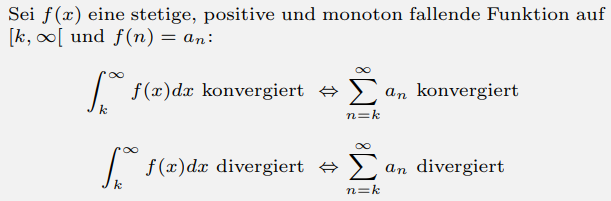
\includegraphics[scale=0.5]{integraltest.png}
\end{KR}

\begin{KR}{Konvergenz Reihen}
    \begin{enumerate}
        \item Handelt es sich um eine spezielle Reihe? (Geometrisch, Teleskopiert, Harmonisch, Zetafunktion)
        \item Ist $\lim a_n$ = 0? (Nullfolgenkriterium)
        \item Ist das Quotientenkriterium oder Wurzelkriterium anwendbar?
        \item Existiert ein konvergierender Majorant / divergirender Minorant?
        \item Kann man das Leibnitzkriterium anwenden?
        \item Integral Test? Partialbruchzerlegung?
    \end{enumerate}
\end{KR}

\begin{center}
    \begin{tikzpicture}[font = \footnotesize]
        \node[draw] (origin) {Gegeben: $\sum_{n=0}^\infty a_n$};
        \matrix (stypes) [
            below = 5mm and 2mm of dstype,
            column sep = 2mm,
            nodes = {
                rectangle,
                draw,
                text width = 18mm,
                minimum height = 12mm
            }
        ] {
            \node[label={[label distance = -4mm]270:geom. Reihe}] (stype1) {$\sum q^n$\\[5pt] $|q| < 1$}; &
            \node[label={[label distance = -4mm]270:altern. Reihe}] (stype2) {$\sum (-1)^n a_n$\\[5pt] $\lim a_n = 0$}; &
            \node[label={[label distance = -4mm]270:Riemann Zeta}] (stype3) {$\zeta (s) = \sum\limits_{n=1}^\infty \frac{1}{n^s}$\\ $s > 1$}; &
            \node[label={[label distance = -4mm]270:Teleskop-Reihe}] (stype4) {$\sum (a_n - a_{n-1})$ \\[5pt] $\exists \lim a_n$}; \\
        };
    \end{tikzpicture}
\end{center}

\subsection{Partialbruchzerlegung bei Reihen}

\noindent Der Grenzwert einer Reihe kann auch mit Partialbruchzerlegung berechnet werden.
\begin{example}
    Was ist der Grenzwert von $\sum_{n=1}^\infty \frac{2}{(n+1)(n+3)}$?
    \tcblower
    \begin{equation*}
        \frac{2}{(n+1)(n+3)} = \frac{a}{n+1} + \frac{b}{n+3} \Rightarrow \begin{cases}
            a + b = 0\\
            3a - b = 2
        \end{cases}
        \quad
        \begin{matrix}
            b = -a = -\frac{1}{2}\\
            a = \frac{1}{2}
        \end{matrix}
    \end{equation*}
    \begin{align*}
        \Rightarrow \sum_{n=1}^\infty \frac{2}{(n+1)(n+3)} &= \frac{1}{2}\sum_{n=1}^\infty\left(\frac{1}{n+1} - \frac{1}{n+3}\right)\\
        & = \frac{1}{2}\left(\frac{1}{2} - \cancel{\frac{1}{4}} + \frac{1}{3} - \cancel{\frac{1}{5}} + \cancel{\frac{1}{4}} - \cancel{\frac{1}{6}} + \ldots\right)\\
        &= \frac{1}{2}\left(\frac{1}{2} + \frac{1}{3}\right) = \frac{5}{2 \cdot 6} = \frac{5}{12}
    \end{align*}
\end{example}
